\section{Background: LLM serving, KVCache, KVCache cache and Multi-turn Serving}
\label{sec:bg}

\begin{figure}[!t]
    %    \vspace{2mm}
        \begin{minipage}{1\linewidth}
        \hspace{-1mm}
        \centering    
        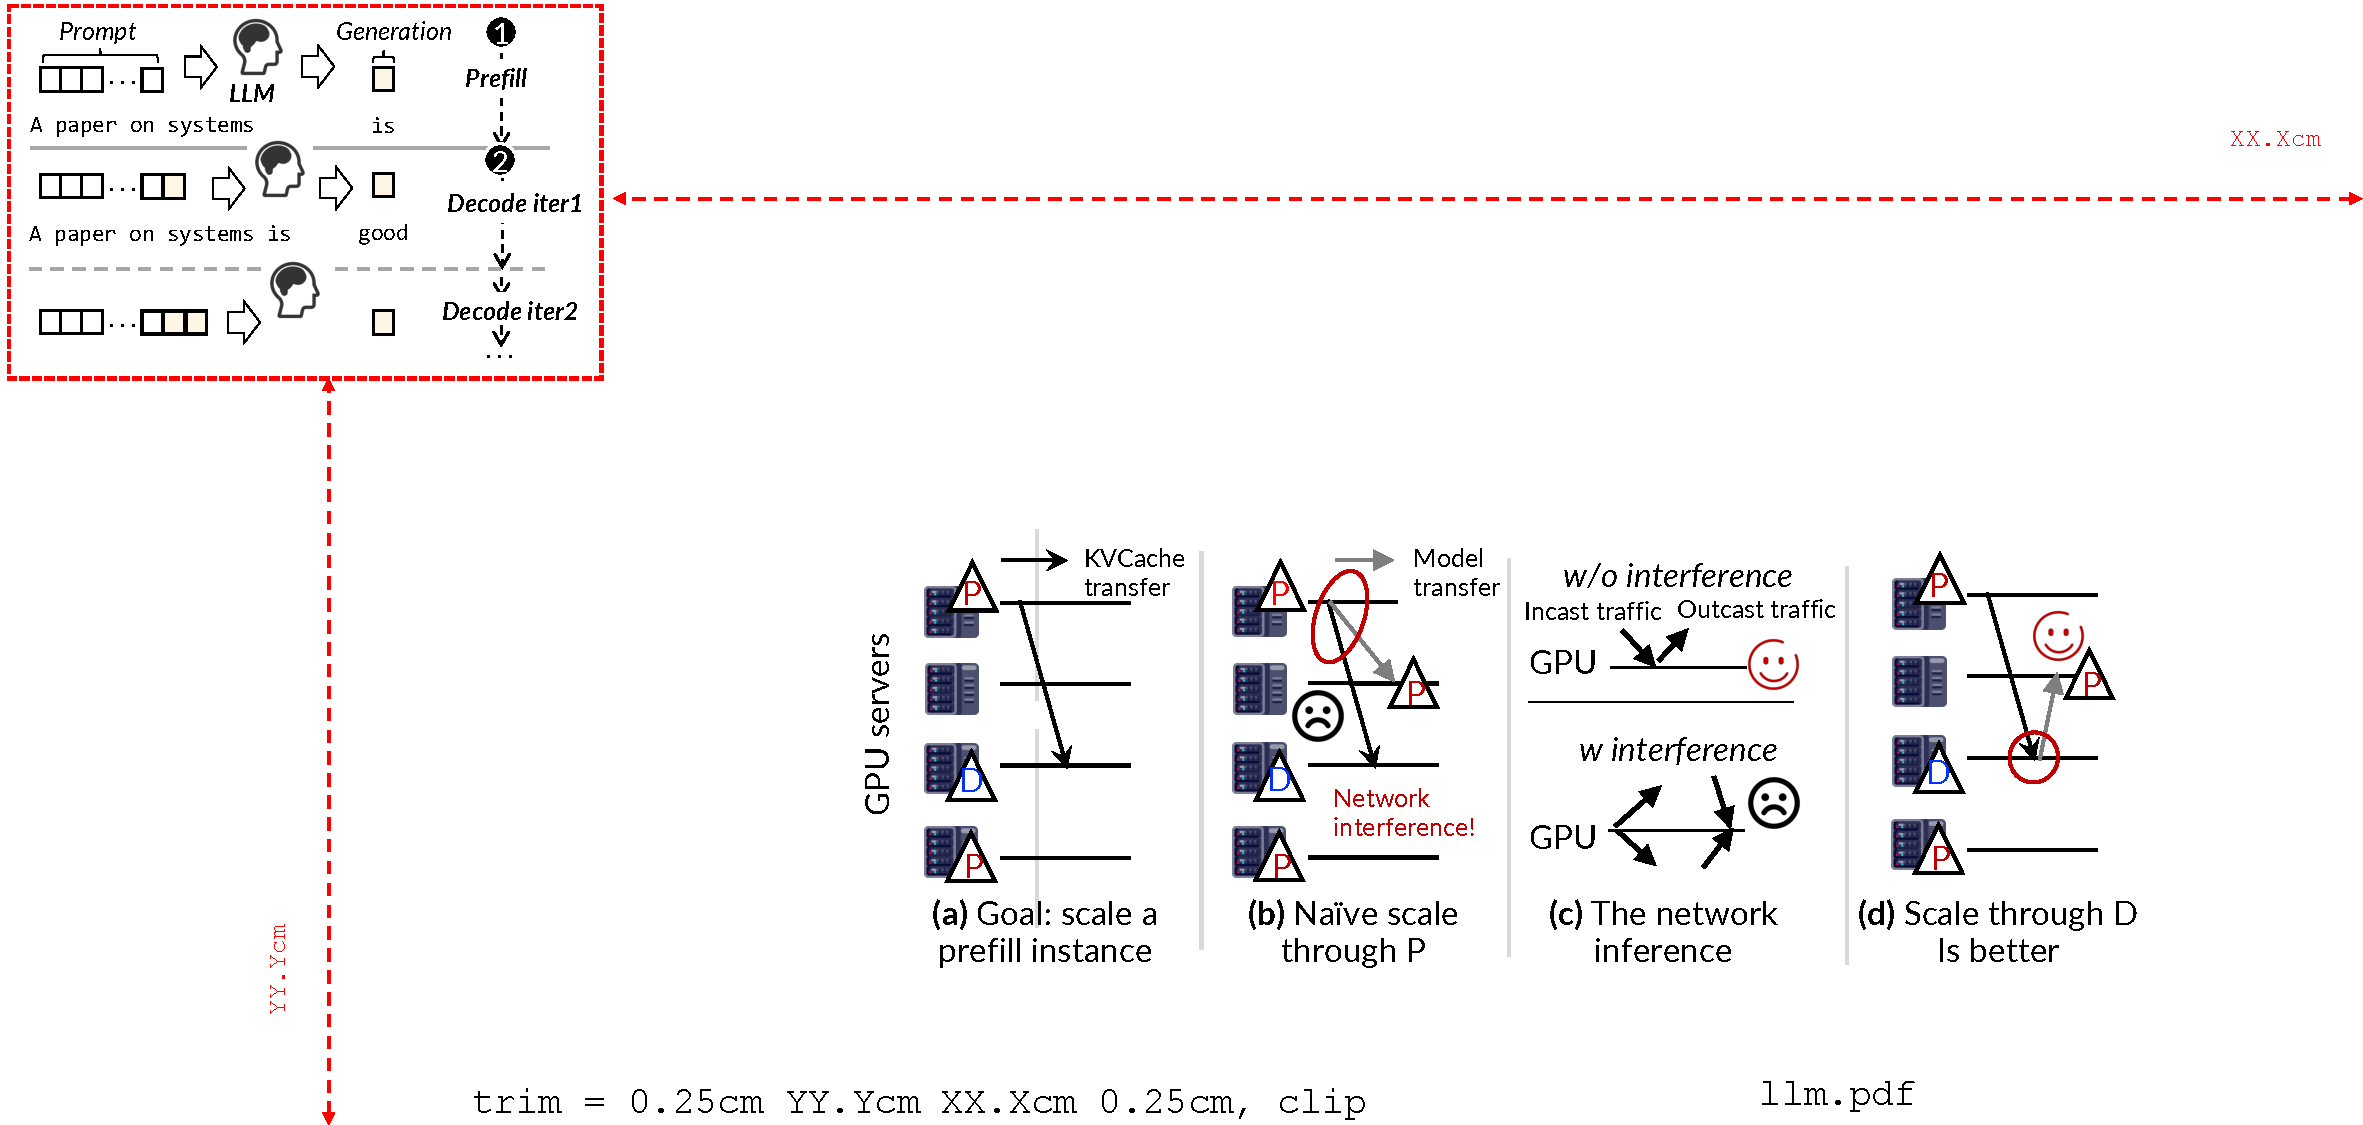
\includegraphics[width=.9\columnwidth, trim=0.25cm 12.7cm 30cm 0.25cm, clip]{figs/llm.pdf} \\[1pt]    
        \end{minipage} \\[1pt]
        \begin{minipage}{1\linewidth}
        \caption{\small{\emph{
            An illustration showing how an LLM processes requests. 
        }}}
        \label{fig:bg-llm}
        \end{minipage} \\[-23pt]
        \end{figure}

\nospacestitle{LLM serving. \,}
Large language models (LLMs) process requests in an auto-regressive way,
as shown in {\fig{fig:bg-llm}}.
Given a request (or a batch of requests),
where each request contains multiple tokens (prompt),
the model first executes a prefill phase to generate the first token (\ding{182})
with a forward pass.
The model then enters a decoding phase (\ding{183})
that iteratively generating the remaining tokens with multiple forward passes.
The iteration ends after the module outputs an end-of-sequence (EOS) token.
During each iteration,
the input consists of both the original prompt and all previously generated tokens.

\begin{figure}[!t]
    %    \vspace{2mm}
        \begin{minipage}{1\linewidth}
        \hspace{-1mm}
        \centering    
        \includegraphics[width=\columnwidth, trim=0.25cm 11.1cm 26.4cm 0.25cm, clip]{figs/kvcache.pdf} \\[1pt]    
        \end{minipage} \\[5pt]
        \begin{minipage}{1\linewidth}
        \caption{\small{ \emph{
        An illustration of: \ding{182} 
        how {\kvcache} from a prefill request (Req\#0) 
        can be reused by the decoding of Req\#0, 
        and \ding{183} how {\kvcache} can be reused for 
        the prefill of a future request (Req\#1). 
        }}}
        \label{fig:bg-kvcache}
        \end{minipage} \\[-10pt]
        \end{figure}

\stitle{KVCache (\kvcache). \,}
LLM performs three steps for a forward pass~\cite{DBLP:conf/nips/VaswaniSPUJGKP17} as shown in {\fig{fig:bg-kvcache}}:
(1) calculating the Q, K, and V matrices using matrix multiplication,
(2) using Q and K to derive attention scores,
and (3) combining the attention scores with the V matrix to produce the attention result.
These steps are computation-intensive.
Since inputs with the same tokens share the same K and V matrices (see \ding{182}),
all LLM serving systems cache the K and V matrices generated during the prefill phase
on the GPUs to save computation time.
These cached K and V matrices are then reused
during the decode phase for the same request to avoid recomputation, so they are termed as {\kvcache}.


\stitle{{\kvcache} cache and {\kvcache} blocks. \,}
Besides {\kvcache} reuse across prefill and decode phases
when processing a single request,
the {\kvcache} can also be reused across different requests
if they share the same token prefix.
As shown in {\fig{fig:bg-kvcache}} (\ding{183}),
the K and V values of ``A paper on''
are identical for both \#Req0 and \#Req1.
Thus, even when \#Req0 finishes decoding,
we can still cache its {\kvcache} for \#Req1,
which dramatically improves the reaction time (also termed time to first token, \emph{TTFT}) of \#Req1:
it only needs to compute the K and V of ``AI is'' during the prefill.
{\kvcache} caching further increases the serving throughput thanks to the saved computation.
Due to the above reasons, existing serving systems all cache the {\kvcache} of completed requests.
We term this approach {\kvcache} cache~\cite{vllm,cachedattention,promptcache,sglang,DBLP:journals/corr/abs-2404-12457,DBLP:conf/sigcomm/LiuLCRHZDY0AMHH24,DBLP:journals/corr/abs-2403-14401},
though other names like prefix cache or prompt cache also exist.
The {\kvcache} can be cached in GPU memory,
on the host memory (or remote machine's memory),
or even SSD~\cite{vllm,cachedattention,DBLP:journals/corr/abs-2403-14401}.

Since checking prefix-match may be costly at a per-token level,
the cache granularity of
existing {\kvcache} system is \emph{block},
where each block contains the KV of a configurable number of tokens.
For example, vLLM~\cite{vllm} by default groups 16 tokens as a block.


\stitle{Multi-turn serving. \,}
Interacting with LLMs through multi-turn conversations is a common pattern
to improve serving quality~\cite{wu2024autogen,wang2023mint}.
Specifically, after receiving the generation from the LLM,
the user may issue a next-turn request with a new prompt. 
Since the LLM needs the previous conversation context for processing, 
the serving system will concatenate the input and output of requests from the previous turns
to the new request's input, and feed the new input to the LLM for serving. 
To help manage the history of multi-turn requests, 
requests in a multi-turn conversation are typically grouped in a \emph{session}.
A multi-turn request naturally reuses {\kvcache} from previous turns 
since current LLM systems deliberately append the history of inputs and outputs 
as a prefix to each new request.